In this section we will show that energy can be extracted from the MP spacetime using the Penrose process. Since the MP spacetime consists of a binary of Reissner-N\"ordstrom constituents, we will use an electrically charged particle to extract electromagnetic energy from the system.

\subsection{Spacetime metric}

For two black holes of masses $M_1$ and $M_2$ and electric charges $Q_1 = M_1$ and $Q_2 = M_2$, in equilibrium and separated by a distance $2a$ along the $z$-axis, the MP line element, in Weyl's cylindrical coordinates, is given by~\cite{SMERAK2016}

\begin{equation}
    \ud s^2 = -U(\rho,z)^{-2} \ud t^2 + U(\rho,z)^2\left[\ud\rho^2 + \rho^2\ud\phi^2 + \ud z^2\right],
    \label{ch:penrose_binaries/ch:penrose_binaries/eq:majumdar_papapetrou_line_element}
\end{equation}
%
where
\begin{equation}
    U(\rho,z) = 1 + \frac{M_1}{\sqrt{\rho^2 + (z+a)^2}} + \frac{M_2}{\sqrt{\rho^2 + (z-a)^2}}.
    \label{ch:penrose_binaries/eq:mp_metric_potential_cylindric}
\end{equation}

The components of the electromagnetic potential $\tens{A}{}{\mu}$ associated with the MP solution are

\begin{equation}
    \tens{A}{}{\mu} = \left(1 - \frac{1}{U}\right)\tens{\delta}{}{\mu t},
    \label{ch:penrose_binaries/eq:electromagnetic_potential_mp}
\end{equation}
%
where $\tens{\delta}{}{\mu\nu}$ is the Kronecker delta.

We remark that Weyl's coordinates describe only the exterior of the black holes, in such a way that their event horizons and their interiors are collapsed into the points $\rho=0, \, z=\pm a$. In particular, due to its staticity, the MP spacetime does not possess an ergosphere (in the usual sense of a spacetime region outside the event horizon where it is impossible for freely-falling particles to ``stand still" -- i.e remain static -- while still being able to escape to infinity). In view of that, and motivated by the possibility of Penrose processes for single charged black holes, instead of analysing geodesic motion we will start by studying the trajectories of charged particles in the MP spacetime.

\subsection{Motion of charged particles}

The motion of a massive charged test particle (with charge-to-mass ratio $\mu$) in any given spacetime with metric $g_{\mu \nu}$ and electromagnetic potential $\tens{A}{}{\mu}$ is governed by the Lagrangian
\begin{equation}
    \mathcal{L} = \frac{1}{2}\mtrtens{\mu}{\nu}\tens{\dot{x}}{\mu}{}\tens{\dot{x}}{\nu}{} - \mu \tens{A}{}{\alpha}\tens{\dot{x}}{\alpha}{},
    \label{ch:penrose_binaries/eq:lagrangian_for_charged_particle}
\end{equation}
%
where $\tens{x}{\mu}{} = \tens{x}{\mu}{}(\lambda) =  \left(t(\lambda), \rho(\lambda), \phi(\lambda), z(\lambda)\right)$ denotes the particle's position (parametrized by its proper time $\lambda$) and dots represent derivatives with respect to $\lambda$. Taking into account the explicit form of the MP metric and of the MP electromagnetic potential, the Lagrangian \eqref{ch:penrose_binaries/eq:lagrangian_for_charged_particle} can be recast as~\cite{RYZNER2015}

\begin{equation}
    \mathcal{L} = \frac{1}{2}\left[-\frac{\dot{t}^2}{U^2} + U^2\left( \dot{\rho}^2 + \rho^2\dot{\phi}^2 + \dot{z}^2 \right) \right] - \mu\left(1-\frac{1}{U}\right)\dot{t}.
    \label{ch:penrose_binaries/eq:explicit_lagrangian_for_charged_particle}
\end{equation}
%
Since the expression above does not depend explicitly on the coordinates $t$ and $\phi$, two constants of motion can be identified, namely the energy divided by the mass of the particle (as measured by a freely-falling observer at infinity),

\begin{equation}
    E \equiv -\del{\mathcal{L}}{\dot{t}} = \frac{\dot{t}}{U^2} + \mu\left(1-\frac{1}{U}\right),
    \label{ch:penrose_binaries/eq:conserved_energy}
\end{equation}
%
and the angular momentum about the $z$ axis divided by the mass of the particle (as measured by a freely-falling observer at infinity),

\begin{equation}
    L \equiv \del{\mathcal{L}}{\dot{\phi}} = U^2 \rho^2 \dot{\phi}.
    \label{ch:penrose_binaries/eq:conserved_momentum}
\end{equation}

Plugging these constants of motion into the 4-velocity normalization condition, $\tens{\dot{x}}{\mu}{}\tens{\dot{x}}{}{\mu} = -1$, and solving for the energy $E$, yields

\begin{equation}
    E = \mu\left(1-\frac{1}{U}\right) + \sqrt{\frac{L^2}{\rho^2U^4} + \frac{1}{U^2} + \dot{\rho}^2 + \dot{z}^2}
    \label{ch:penrose_binaries/eq:alternative_expression_for_energy},
\end{equation}
where the negative root has been neglected due to the fact that $E$ must be positive at infinity when $\mu = 0$ (for a detailed discussion about positive and negative root states for $E$ see Ref. \cite{RUFFINI1971}). We note that Eq.~\eqref{ch:penrose_binaries/eq:alternative_expression_for_energy} reduces to the expression found in Ref.~\cite{DENARDO1973} for a Reissner-Norstr{\"o}m black hole if the mass of one of the black holes is taken to be zero and an appropriate coordinate system, centered around the other black hole, is used.

Finally, the equations of motion are obtained directly from the Euler-Lagrange equations. After using \myref{ch:penrose_binaries/eq:conserved_energy} and \myref{ch:penrose_binaries/eq:conserved_momentum} to eliminate $\dot{t}$ and $\dot{\phi}$ from the resulting expressions, one is left with

\begin{multline}
    \ddot{\rho}-\frac{L^2(U+\rho\indexdel{\rho}U)}{\rho^3 U^5} + \frac{2\dot{\rho}\dot{z}\indexdel{z}U - (E^2 + \dot{z}^2 - \dot{\rho}^2)\indexdel{\rho}U}{U} \\- \frac{\mu}{U}\left(\mu-2E+\frac{E-\mu}{U}\right)\indexdel{\rho}U = 0,
    \label{ch:penrose_binaries/eq:ode_for_rho_motion}
\end{multline}
%
and
\begin{multline}
    \ddot{z}-\frac{L^2\indexdel{z}U}{\rho^2 U^5} + \frac{2\dot{\rho}\dot{z}\indexdel{\rho}U - (E^2 - \dot{z}^2 + \dot{\rho}^2)\indexdel{z}U}{U} \\- \frac{\mu}{U}\left(\mu-2E+\frac{E-\mu}{U}\right)\indexdel{z}U = 0,
    \label{ch:penrose_binaries/eq:ode_for_z_motion}
\end{multline}
which reduce to the equations of motion found in Ref.~\cite{ASSUMPCAO2018} for neutral particles. Together with Eqs.~\eqref{ch:penrose_binaries/eq:conserved_energy} and \eqref{ch:penrose_binaries/eq:conserved_momentum}, the two equations above fully determine the trajectory of a massive charged particle in the MP spacetime once appropriate initial conditions have been specified.

\subsection{Generalized ergosphere}

The possibility of extracting energy from a black hole through the Penrose mechanism is intimately linked to the existence of negative-energy trajectories (as measured by observers far away from the black hole). As explained before, in the MP spacetime (and in other static spacetimes like Reissner-Nordstrom) there are no ergospheres in the usual sense, meaning that geodesic motion is always associated with positive energy trajectories. Any charged particle moving through the MP spacetime, however, will be affected by Lorentz forces from its electromagnetic interaction with the black holes and, consequently, will satisfy the equations of motion derived in the previous section. Even though there are no ergospheres in MP, since the trajectories associated with Eqs.~\eqref{ch:penrose_binaries/eq:conserved_energy}, \eqref{ch:penrose_binaries/eq:conserved_momentum}, \eqref{ch:penrose_binaries/eq:ode_for_rho_motion} and \eqref{ch:penrose_binaries/eq:ode_for_z_motion} are not geodesics, negative values for the constant of motion $E$ are not forbidden \emph{a priori}. If negative energy trajectories exist in the MP spacetime, then one can define generalized ergospheres as the regions of spacetime where they are allowed to exist. The concept of generalized ergospheres is not new, however, and was first introduced by Denardo and Ruffini for the Reissner - Nordstr\"om solution in Ref.~\cite{DENARDO1973}, where they have additionally shown that the Penrose process is viable in this spacetime by presenting concrete examples. That being said, defining a generalized ergosphere for the MP spacetime is a natural step forward from D. and R. since it consists of two extremely charged RN black holes.

From Eq.~\eqref{ch:penrose_binaries/eq:alternative_expression_for_energy} it is evident that, for fixed $\mu$, the energy is completely determined by the angular momentum $L$, and the values of $\rho$, $z$, $\dot{\rho}$ and $\dot{z}$  at any given instant of time. Therefore, at a fixed position in space, the minimum possible energy is associated with particles at rest. Letting $\dot{\rho}=\dot{z}=0$ and $L=0$ (i.e.~$\dot{\phi}=0$), we conclude that the minimum energy $E_{\mathrm{min}}$ for a particle, as a function of its position, is
\begin{equation} \label{ch:penrose_binaries/eq:minimum_energy}
    E_{\mathrm{min}} = \mu\left(1-\frac{1}{U}\right) + \frac{1}{U}.
\end{equation}

By requiring the minimum energy to be negative, we find that $\mu$ must necessarily be negative (which means that the particle's charge is opposite to the charge of the black holes) and that the particle (at rest) must be inside the spatial region determined by
\begin{equation} \label{ch:penrose_binaries/eq:negative_energy_condition}
    \frac{M_1}{\sqrt{\rho^2 + (z+a)^2}} + \frac{M_2}{\sqrt{\rho^2 + (z-a)^2}} > - \frac{1}{\mu}.
\end{equation}

Since $\mu$ is a dimensionless quantity, it makes sense to recast the left side of \eqref{ch:penrose_binaries/eq:negative_energy_condition} as a dimensionless quantity as well so that we are comparing two pure numbers. To do so, one must simply divide both numerators and denominators of the left side of the inequality by, say, $M_1$ and define $\overline{\rho} \equiv \rho/M1$, $\overline{z} \equiv z/M1$, $M \equiv M_1/M_2$, $\alpha = a/M1$ to obtain

\begin{equation} \label{ch:penrose_binaries/eq:rescaled_negative_energy_condition}
    \frac{1}{\sqrt{\overline{\rho}^2 + (\overline{z}+\alpha)^2}} + \frac{M^{-1}}{\sqrt{\overline{\rho}^2 + (\overline{z}-\alpha)^2}} > - \frac{1}{\mu}.
\end{equation}

This last inequality determines the generalized ergosphere of the MP spacetime as a region depending only on three dimensionless parameters: $M$, $\alpha$ and $\mu$. Particles with charge-to-mass ratio $\mu$ inside the region determined by \eqref{ch:penrose_binaries/eq:rescaled_negative_energy_condition} can have negative energies, while particle outside will never have negative energies. Note that this notion of ergosphere depends not only on the geometry of the spacetime, but also on properties of the particle.

In order to have a graphical representation of the generalized ergosphere, let us use cartesian-like coordinates, also reescaled by $M_1$, $(\overline{x},\overline{y},\overline{z})$ related to Weyl's coordinates by $\overline{x}=\overline{\rho} \cos \phi$ and $\overline{y}=\overline{\rho} \sin \phi$. In Figs.~\ref{ch:penrose_binaries/fig:splitting_1}-\ref{ch:penrose_binaries/fig:splitting_4}, we plot the generalized ergosphere for a MP black hole binary of unitary mass-ratio $M$, whose horizons (represented by red dots) have also unitary separation parameter $\alpha$. As the value of $\mu$ increases, one can observe that the generalized ergosphere splits into two disconnected spherical regions with the same (albeit smaller than the original) radius. Thus we see that the bigger the value of $\mu$, the closer to the horizon an orbit must be in order to realize energy extraction. Extrapolating this result makes it easy to see that the maximum possible amount of energy can only be extracted if a particle is orbiting exactly \emph{at} the event horizon. We will explore this fact further in another section of this work but this result is in agreement with~\cite{RUFFINI1971}.

In Figs.~\ref{ch:penrose_binaries/fig:mass_increase_1}-\ref{ch:penrose_binaries/fig:mass_increase_2}, we turn to the influence of the mass-ratio in the generalized ergosphere's shape while keeping fixed $\mu = -1$ and $\alpha = 1$. The ergosphere starts of with the same shape as in Fig.~\ref{ch:penrose_binaries/fig:splitting_1}. As the mass-ratio increases, the ergosphere around one of the black holes is enlarged while the other's shrunken until a split-up occurs, and again, one ends up with two disconnected regions but this time of different sizes, the larger of which is centered around the heavier black hole. Again, this is to be expected. Because the MP solution represents extremally charged black holes, as the mas of the objects increase (or decrease) so does their electric charge thus allowing for more energy to be extracted and consequently a larger generalized ergosphere.

Finally, in Figs.~\ref{ch:penrose_binaries/fig:distance_1}-\ref{ch:penrose_binaries/fig:distance_2} we show the effects on the generalized ergosphere resulting from the increase in the distance parameter $\alpha$ with $M=1$ and $\mu=-1$ fixed. Initially the ergosphere is shaped as in Fig.~\ref{ch:penrose_binaries/fig:splitting_1}. Yet again, as the value of $\alpha$ increases, the ergosphere becomes elongated along the $z$ direction, assuming a `peanut'-like shape until it is split into two disconnected regions. From \eqref{ch:penrose_binaries/eq:rescaled_negative_energy_condition}, we can verify that the splitting occurs when $\alpha = -(M^{-1}+1)\mu$. If the black holes are moved further apart, the system will eventually behave as two isolated extremal black holes of mass $M$, each one surrounded by its own spherical generalized ergosphere.

It's also very important to point out that for small separations the generalized ergosphere of the binary system becomes equal to the one around a single RN black hole of mass $M_1 + M_2$. One can easily see that by taking the limit $a \rightarrow 0$ in \eqref{ch:penrose_binaries/eq:negative_energy_condition} and going to spherical coordinates, related to Weyl's coordinates trough $\rho = \sin\theta$ and $z=r\cos\theta$, which leads to the conclusion that that the generalized ergosphere is the spherical region centered around the origin which satisfies $r < -\mu (M_1 + M_2).$ This is precisely the same region as the one presented in Eq. (12) of Ref.~\cite{DENARDO1973} if one considers an extremal black hole in coordinates such that the event horizon is a point at the origin (which amounts the transformation $r \rightarrow r + M$) with the RN solution's mass parameter $M$ replaced by the total mass of the binary system, $M_1 + M_2$.

\begin{figure}[!htbp]
    \centering
    \subfloat[$\mu=-1$]{
        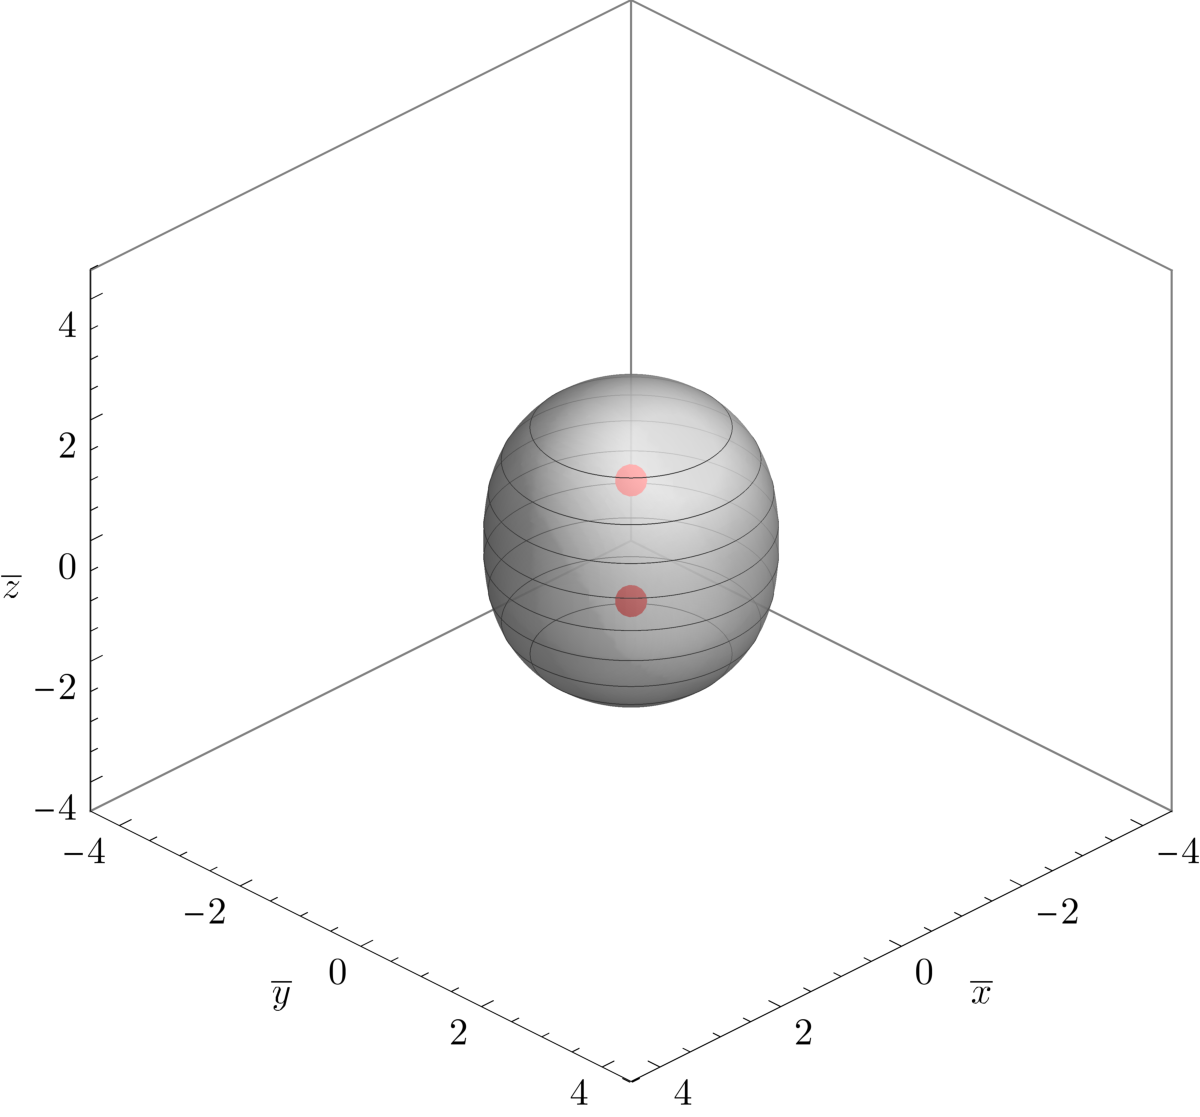
\includegraphics[width = 0.43\linewidth]{img/penrose_binaries/mp/ergo_1.pdf}
        \label{ch:penrose_binaries/fig:splitting_1}
    }
    \subfloat[$\mu=-0.6$]{
        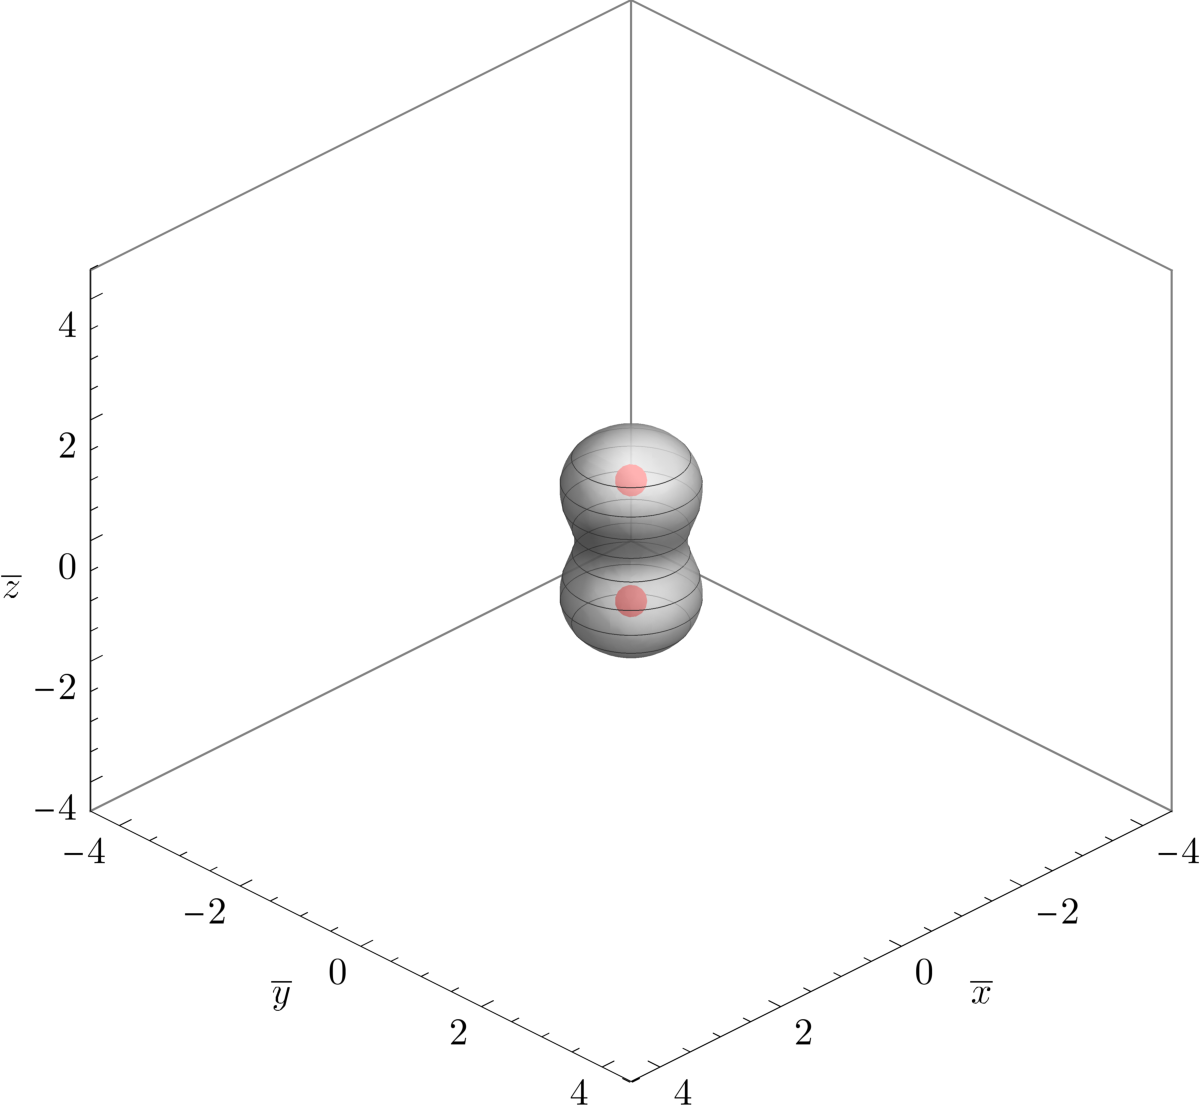
\includegraphics[width = 0.43\linewidth]{img/penrose_binaries/mp/ergo_2.pdf}
        \label{ch:penrose_binaries/fig:splitting_2}
    }
    \newline
    \subfloat[$\mu=-0.5$]{
        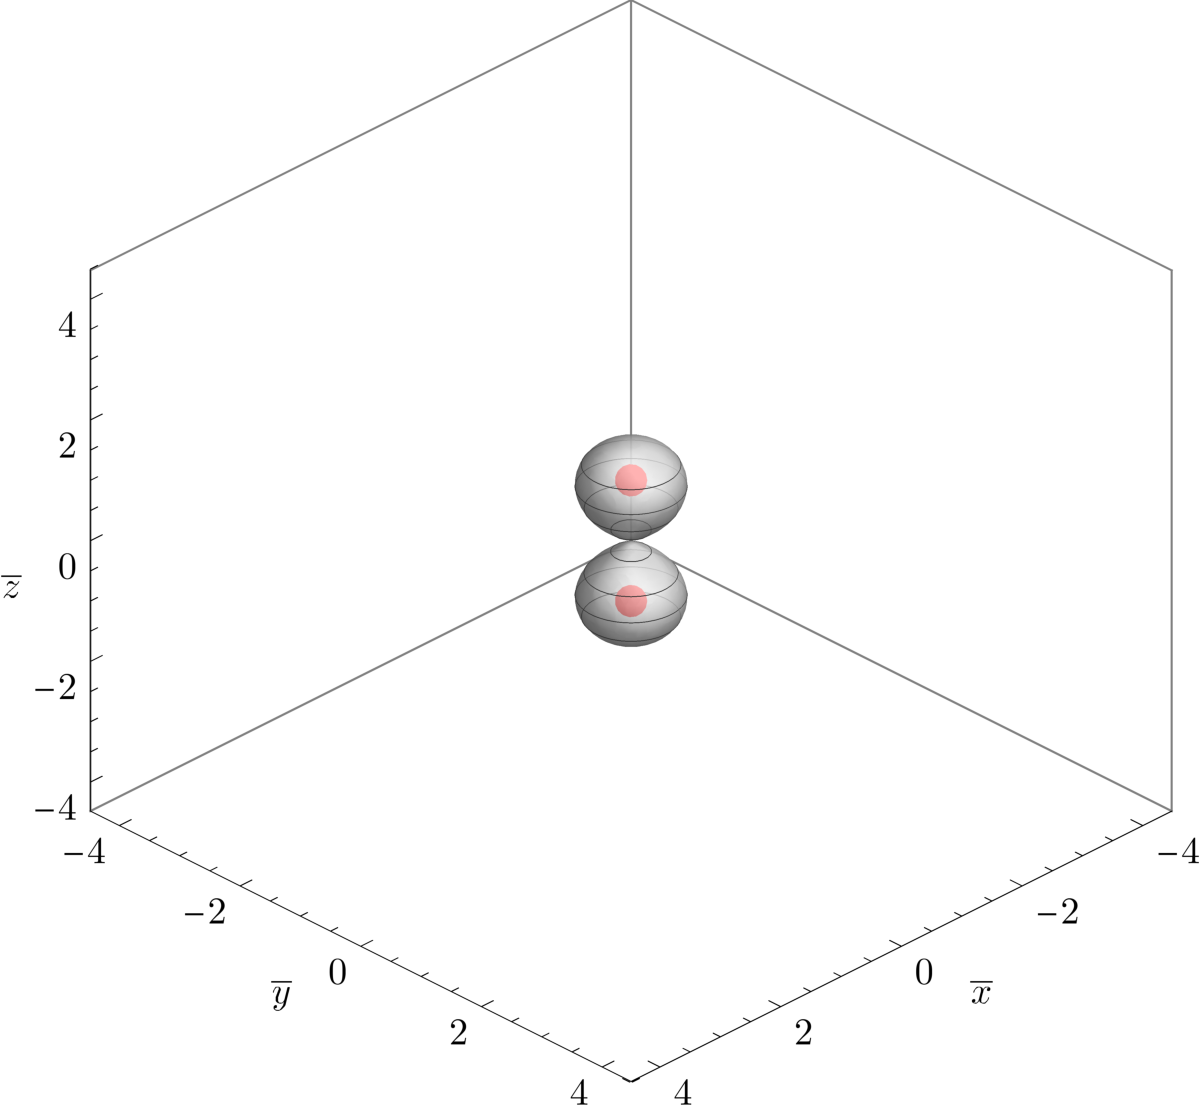
\includegraphics[width = 0.43\linewidth]{img/penrose_binaries/mp/ergo_3.pdf}
        \label{ch:penrose_binaries/fig:splitting_3}
    }
    \subfloat[$\mu=-0.35$]{
        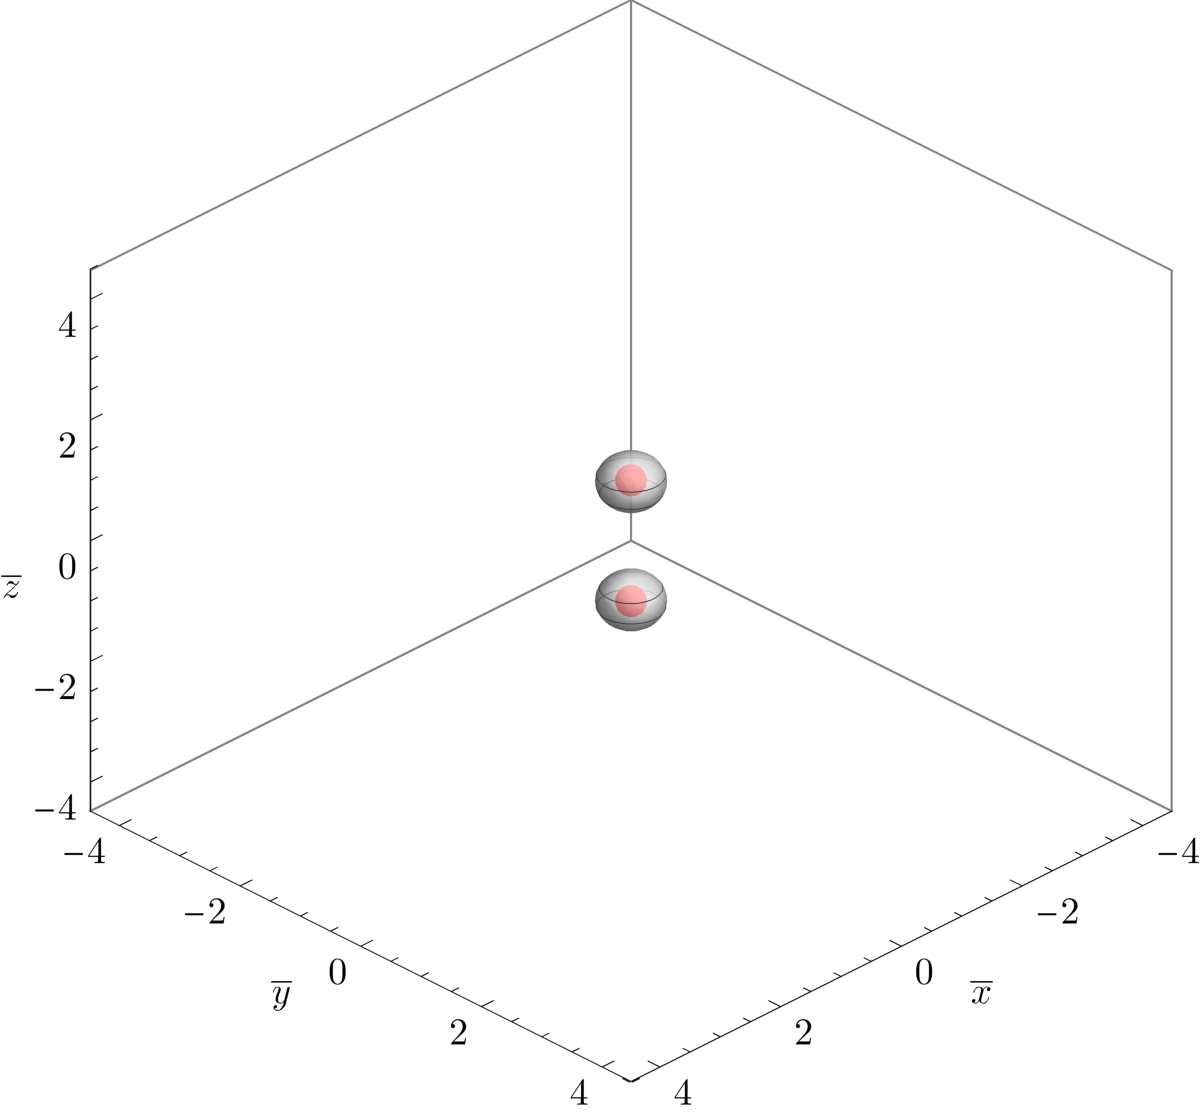
\includegraphics[width = 0.43\linewidth]{img/penrose_binaries/mp/ergo_4.pdf}
        \label{ch:penrose_binaries/fig:splitting_4}
    }
    \caption{Splitting and shrinking of the generalized ergosphere caused by an increase in the charge-to-mass ratio $\mu$ of a test particle. The separation parameter and mass-ratio are kept fixed at $\alpha = 1$ and $M = 1$, respectively. Note that the splitting produces two symmetric regions that are closer to the horizons.}
    \label{ch:penrose_binaries/fig:splitting_ergosphere_mass_increase}
\end{figure}

\begin{figure}[!htbp]
    \centering
    \subfloat[$M=2$]{
        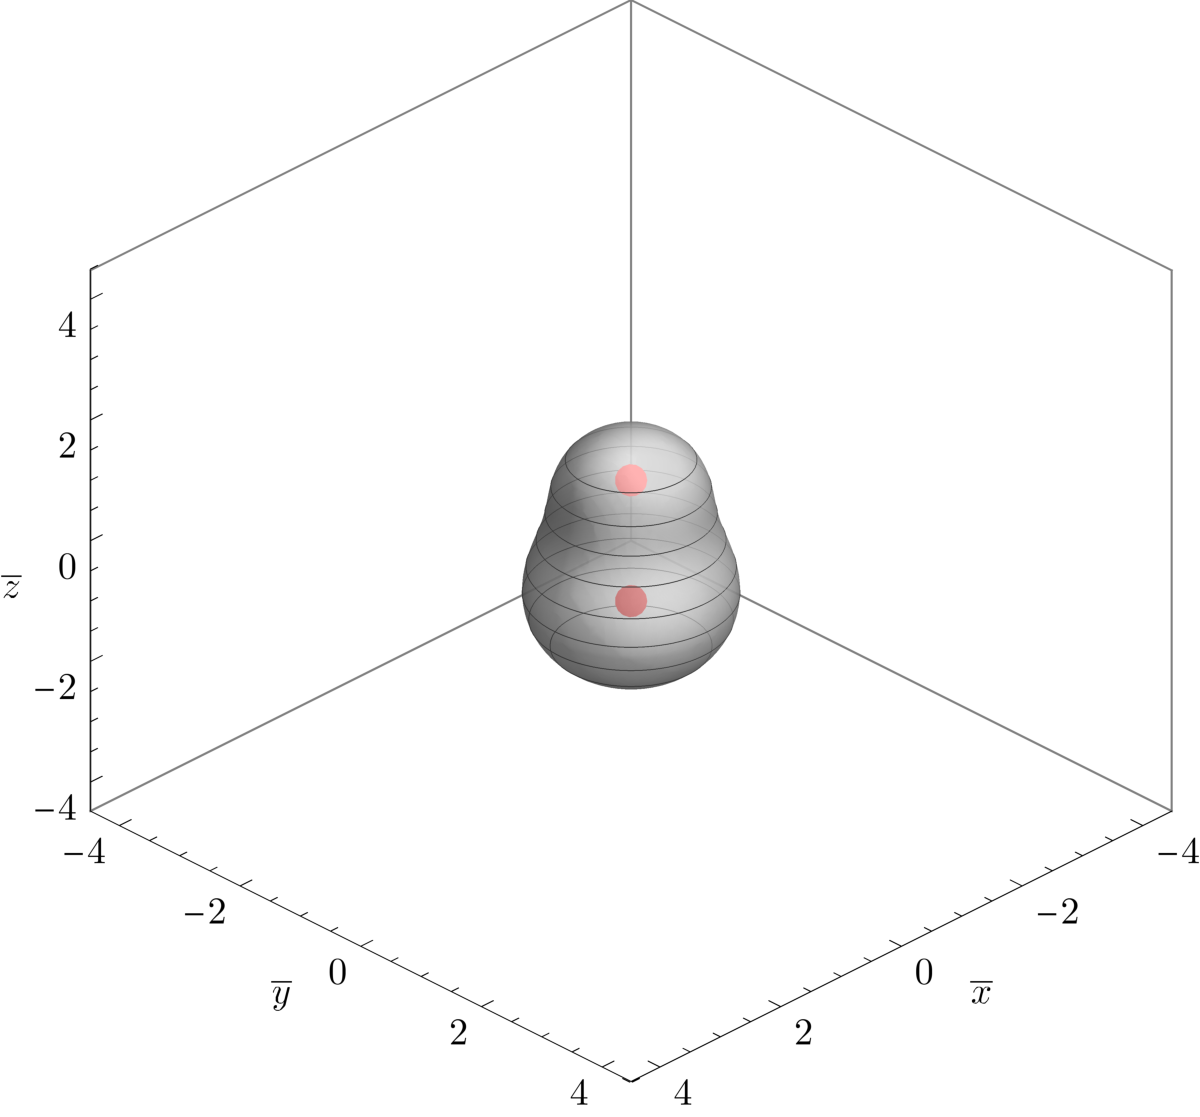
\includegraphics[width = 0.43\linewidth]{img/penrose_binaries/mp/ergo_5.pdf}
        \label{ch:penrose_binaries/fig:mass_increase_1}
    }
    \subfloat[$M=20/3$]{
        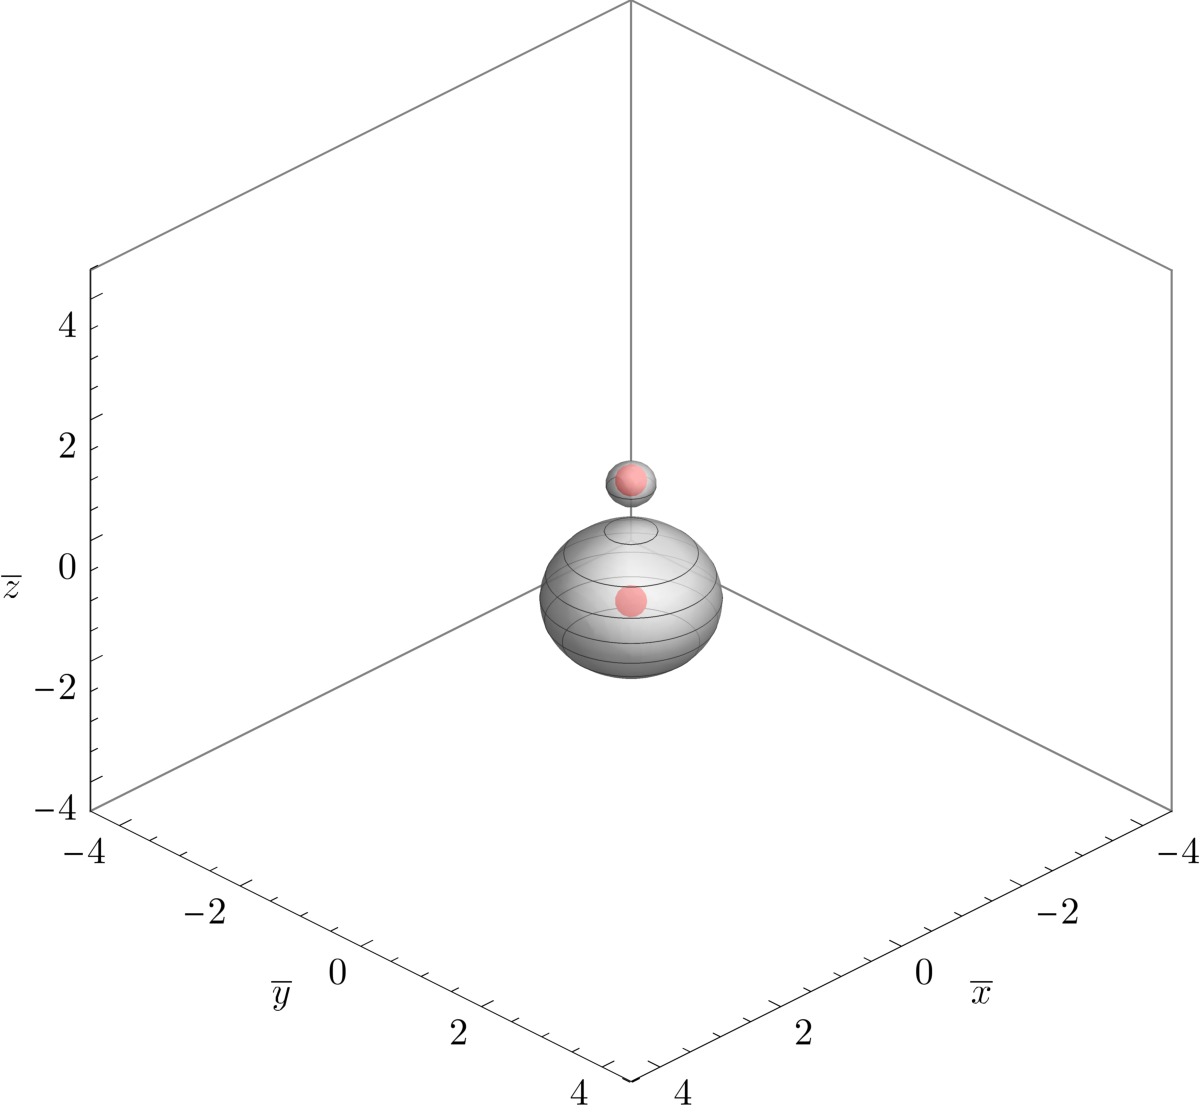
\includegraphics[width = 0.43\linewidth]{img/penrose_binaries/mp/ergo_6.pdf}
        \label{ch:penrose_binaries/fig:mass_increase_2}
    }
    \caption{Splitting of the generalized ergosphere caused by an increase in the mass ratio $M$. The separation parameter and charge-to-mass ratio are kept fixed at $\alpha = 1$ and $\mu = -1$, respectively. The final region is much larger around the heavier black hole.}
    \label{ch:penrose_binaries/fig:splitting_ergosphere_mass_increase}
\end{figure}

\begin{figure}[!htbp]
    \centering
    \subfloat[$\alpha=2$]{
        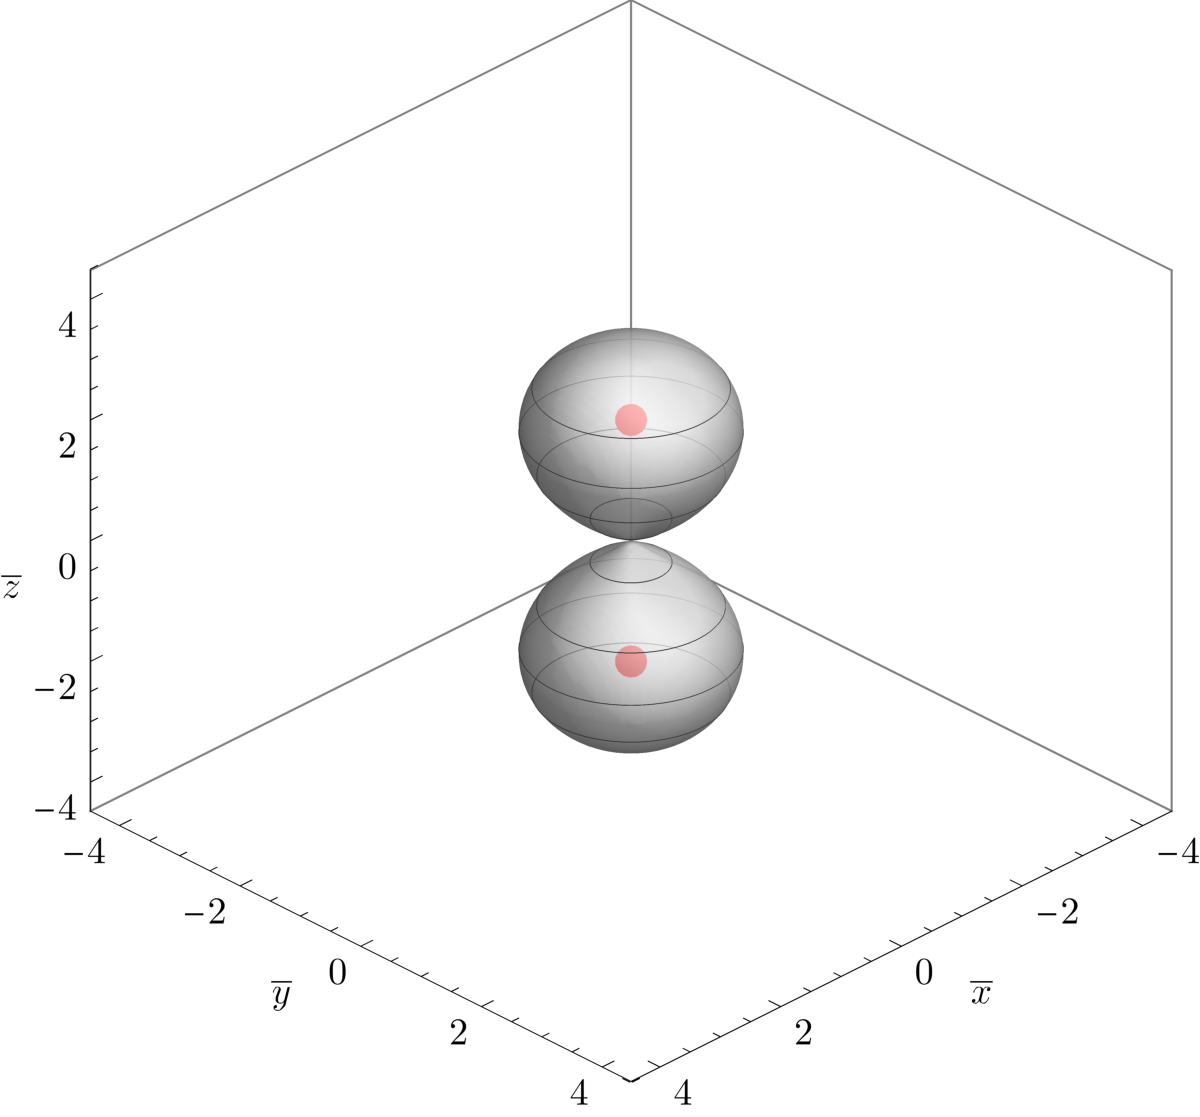
\includegraphics[width = 0.43\linewidth]{img/penrose_binaries/mp/ergo_7.pdf}
        \label{ch:penrose_binaries/fig:distance_1}
    }
    \subfloat[$\alpha=3$]{
        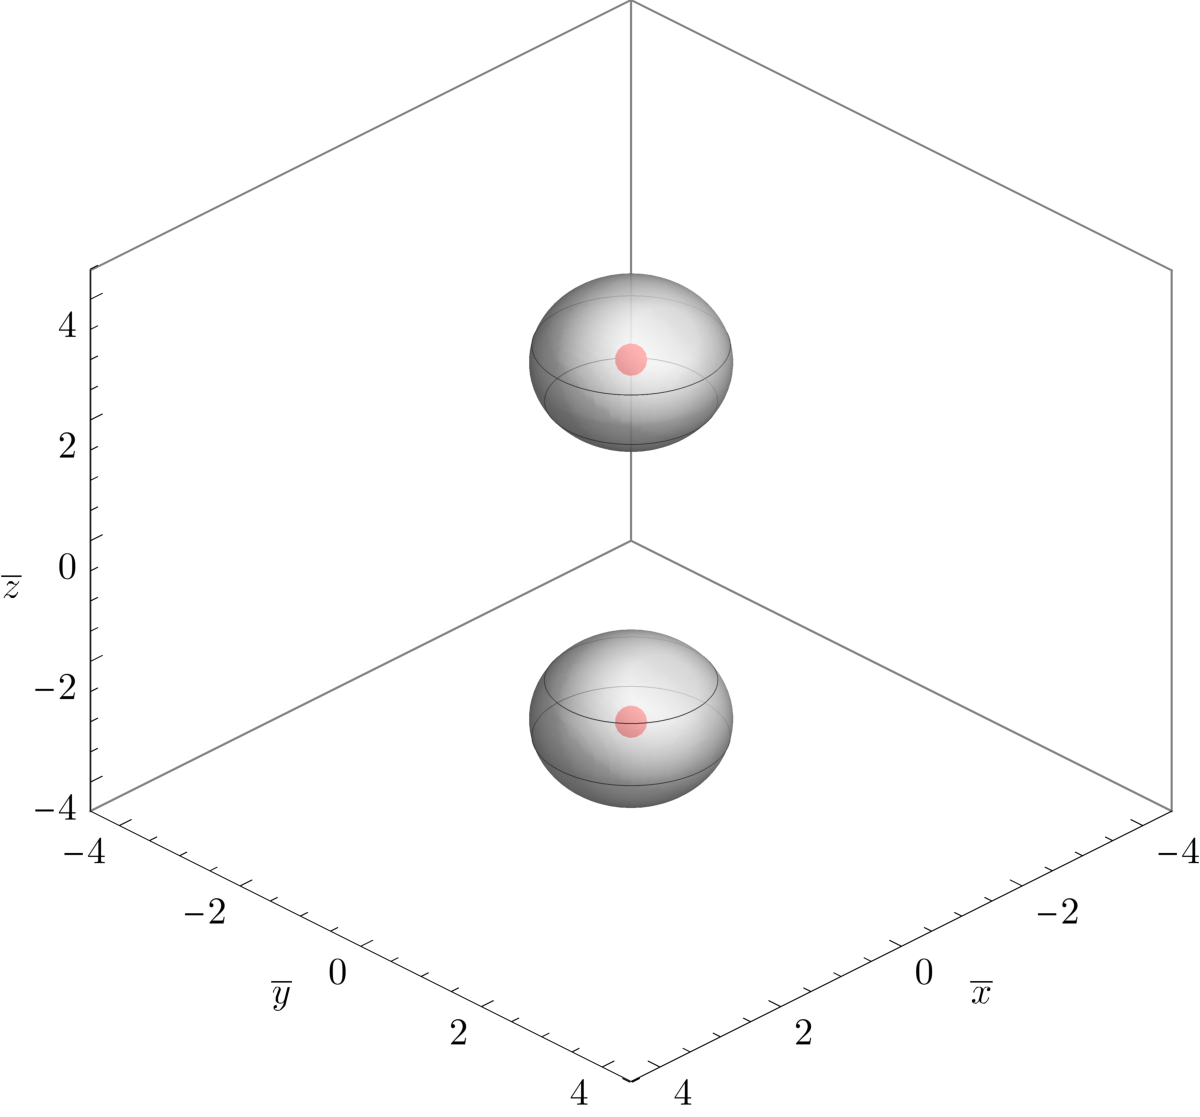
\includegraphics[width = 0.43\linewidth]{img/penrose_binaries/mp/ergo_8.pdf}
        \label{ch:penrose_binaries/fig:distance_2}
    }
    \caption{Splitting of the generalized ergosphere caused by an increase in the distance parameter $\alpha$ The mass ratio and charge-to-mass ratio are kept fixed at $M = 1$ and $\mu = -1$, respectively. The split region is symmetric and it is not closer farther than it previously was to either horizon.}
    \label{ch:penrose_binaries/fig:splitting_ergosphere_distance_increase}
\end{figure}

\subsection{Negative energy orbits and the Penrose process}

Having understood the notion of generalized ergospheres around binary black holes described by the MP metric, we are now in position to analyze the possibility of energy extraction in such spacetimes. The idea follows Penrose's original proposal~\cite{PENROSE1971} and its extension to RN black holes~\cite{RUFFINI1971,DENARDO1973}. The mechanism we shall explore consists in sending a negatively charged particle from sufficiently far away towards the binary black hole.  Once the particle enters the generalized ergosphere, we need it to break up into two pieces. Depending on how the splitting process is set up, one of the pieces will escape back to infinity with more energy than the incident particle had.

In order to accomplish this one needs three trajectories. The first one, with positive energy $E^{(0)} > 0$ and labeled $T^{(0)}$, must start outside the ergosphere and end inside it, at the point where the other two trajectories, labeled $T^{(1)}$ and $T^{(2)}$ start. One of them, let us say $T^{(1)}$, must have negative energy, i.e.~$E^{(1)}<0$, and, therefore, will remain confined inside the ergosphere. The other one, $T^{(2)}$, on the other hand, will have positive energy $E^{(2)} > E^{(0)}$, which allows it to escape the ergospohere and reach back infinity.

Suppose that the break-up of the particle occurs at $(\rho_0,\phi_0,z_0)$. Let $m^{(i)}$ and $\tens{P}{(i)}{\mu}$ denote, respectively, the mass and the the 4-momentum of the particle on trajectory $T^{(i)}$. The conservation of the four-momentum, applied at the break-up point, reads
\begin{equation}
    \tens{P}{(0)}{\mu} = \tens{P}{(1)}{\mu} + \tens{P}{(2)}{\mu}.
    \label{ch:penrose_binaries/eq:four_momentum_conservation}
\end{equation}
%
Each component of the vector equation above yields a different conservation equation with straightforward physical interpretation. The zero-component, for a start, is just the conservation of total energy, i.e.
\begin{equation}
    m^{(0)}E^{(0)} = m^{(1)}E^{(1)} + m^{(2)}E^{(2)},
    \label{ch:penrose_binaries/eq:conservation_of_charge_energy}
\end{equation}
while the angular component is simply the conservation of angular momentum around the $z$ axis, namely
\begin{equation}
    m^{(0)}L^{(0)} = m^{(1)}L^{(1)} + m^{(2)}L^{(2)}.
    \label{ch:penrose_binaries/eq:conservation_ang_mom}
\end{equation}
The other two components represent the conservation of linear momentum along the radial direction and along the $z$ axis, respectively
\begin{equation}
    \tens{m}{(0)}{}\tens{\dot{\rho}}{(0)}{} = \tens{m}{(1)}{}\tens{\dot{\rho}}{(1)}{} + \tens{m}{(2)}{}\tens{\dot{\rho}}{(2)}{}
    \label{ch:penrose_binaries/eq:conservation_rho}
\end{equation}
%
and
%
\begin{equation}
    \tens{m}{(0)}{}\tens{\dot{z}}{(0)}{} = \tens{m}{(1)}{}\tens{\dot{z}}{(1)}{} + \tens{m}{(2)}{}\tens{\dot{z}}{(2)}{},
    \label{ch:penrose_binaries/eq:conservation_z}
\end{equation}

where all the derivatives are to be evaluated at the break-up point $(\rho_0,\phi_0,z_0)$.

Because we've assumed that $E^{(1)} < 0$, it's easy to see from \eqref{ch:penrose_binaries/eq:conservation_of_charge_energy} that the particle on trajectory $T^{(2)}$ will be more energetic than the particle on trajectory $T^{(0)}$ and thus it has \emph{gained} energy during the split-up process. Obviously this extra energy must come from somewhere. In Penrose's original proposal, the extra energy came from a small loss of angular momentum in the background Kerr black hole. This idea can be readily extended to charged black holes: now instead of angular momentum, the black hole donates part of it's electromagnetic energy to an outgoing particle. One might naturally ask how much energy can be extracted using this process. This was not answered by Penrose but by Christodoulou in Ref.~\cite{CHRISTODOULOU1970}. It turns out that the mass of a black hole cannot be smaller than a certain \emph{irreducible mass}, and about 50\% of a charged black hole's electromagnetic energy and 29\% of a rotating black hole's angular momentum can be extracted through this process. An important variation of the Penrose process is to consider particle collisions, instead of break-ups. This is befittingly known as the collisional Penrose process and it is capable of producing much more energetic ejecta that could be a potential source of gamma rays and high energy cosmic rays (see e.g.~\cite{PhysRevLett.114.251103}), however, in our work we will only focus on the non-colisional version the Penrose process.

The existence of a generalized ergosphere as we've shown, indicates that negative energy orbits can exist and thus electromagnetic energy can be extracted from a MP binary through the Penrose process. However we are not only interested in where these orbits are located but also on some of their features, e.g., weather they fall into one of the black holes or keep orbiting the system in a closed orbit. In the following sections we will describe briefly the characteristics of negative energy orbits constrained to two planes of motion around the system. This analysis will come into play later when we construct two explicit examples of the penrose process in action. We start by introducing two quantities, the \emph{effective energy} $E_{\text{eff}}(\rho,z)$ and the \emph{effective potential} $V_{\text{eff}}(\rho,z)$, given by

\begin{equation}
    E_{\text{eff}}(\rho,z) \equiv E - \mu\left(1 - \frac{1}{U(\rho,z)}\right)
    \label{ch:penrose_binaries/eq:effective_energy_definition}
\end{equation}
%
and

\begin{equation}
    V_{\text{eff}}(\rho,z) \equiv \frac{L^2}{\rho^2 U(\rho,z)^4} + \frac{1}{U(\rho,z)^2}.
    \label{ch:penrose_binaries/eq:effective_potential_definition}
\end{equation}

With that, we can recast Eq.~\eqref{ch:penrose_binaries/eq:alternative_expression_for_energy} as

\begin{equation}
    \dot{\rho}^2 + \dot{z}^2 = E_{\text{eff}}(\rho,z)^2 - V_{\text{eff}}(\rho,z).
    \label{ch:penrose_binaries/eq:first_order_ode_for_orbits}
\end{equation}

\subsubsection{Orbits in the \texorpdfstring{$\rho$}{$\symit{rho}$}-$z$ plane}

One can easily see that by setting $L$ (and thus $\dot{\phi}$) to zero, the particle's orbit will be constrained to a plane that contains both of the black holes, which we call the $\rho$-$z$ plane. Because of the system's cylindrical symmetry one can set $\phi = 0$ without any loss of generality. To be able to integrate the equations of motion \eqref{ch:penrose_binaries/eq:ode_for_rho_motion} and \eqref{ch:penrose_binaries/eq:ode_for_z_motion} one must specify the remaining 4 initial conditions for $\rho$, $z$ and their time derivatives. Note however that $E$, $\dot{\rho}$ and $\dot{z}$ are related trough \eqref{ch:penrose_binaries/eq:first_order_ode_for_orbits} and thus it suffices to choose $\rho(0)$, $z(0)$, $\dot{z}(0)$ and $E$ while using \eqref{ch:penrose_binaries/eq:first_order_ode_for_orbits} to determine $\dot{\rho}(0)$.

In order to visualize the orbits we employ once again Cartesian-like coordinates $(\overline{x},\overline{y},\overline{z})$ reescaled by $M_1$, $M$ as the system's mass-ratio and $\alpha$ as it's separation parameter. In Figs.~\ref{ch:penrose_binaries/fig:orbit_1} and \ref{ch:penrose_binaries/fig:orbit_2} the event horizons are represented by black dots and the spacetime parameters were fixed at $M = \alpha = 1$. Additionally, because our process for finding $\dot{\rho}(0)$ involves square roots we use solid black lines for orbits resulting from the positive solution and dashed black lines for the negative solution. By extensively testing for many different initial conditions, we found that most orbits end up in either of the two black holes as in Fig.~\ref{ch:penrose_binaries/fig:orbit_1}. This is not surprising, as particles that follow negative energy orbits must always be charged oppositely to the black holes and thus they will always be electrically attracted towards the horizons. On the other hand, by choosing parameters very carefully, one is be able to find highly unstable but closed orbits as in Fig.~\ref{ch:penrose_binaries/fig:orbit_2}.

At a first glance, closed negative energy orbits might cause some concern as they never fall into one of the horizons and thus never effectively interact with the black holes to cause them to loose a small amount of electric charge but one must keep in mind that in the MP spacetime such orbits are always unstable and are completely within the generalized ergosphere. Additionally, the existence of closed negative energy orbits is not an exclusive feature of the MP metric. Usually these orbits occur only \emph{inside} event horizons or in naked singularities. Stuchlik has shown in Ref.~\cite{STUCHLIK1980} that there can exist stable circular orbits of negative energy around a Kerr naked singularity and that the Penrose process can effectively take place using said orbits. Patil and collaborators in Ref.~ \cite{PATIL2016} have even used this fact to construct a model to explain the origin of ultra high energy particles detected on Earth as a result of the colisional Penrose process in a slightly over spinning Kerr black hole. Similarly, Mukherjee and Nayak  in Ref.~\cite{MUKHERJEE2018} have used the colisional Penrose process in a Kerr naked singularity with orbits outside the equatorial plane to construct a model for energetic outgoing particle jets. In some situations though, closed negative energy orbits can exist outside of the event horizon as Prasana and Dadhich have shown in Ref.~\cite{PRASANA1982} in the spacetime of a Kerr black hole immersed in an external magnetic field that is regular up to the event horizon. More recently Felice and collaborators in Ref.~\cite{FELICE2004} also have shown that magnetized particles in a Kerr black hole can give rise to stable circular orbits of negative energy inside the ergosphere. Therefore, these unstable orbits that we've found are not violating any underlying fundamental principle.

\begin{figure}[!htbp]
    \centering
    \subfloat[$\overline{\rho}(0) = 0$, $\overline{z}(0) = 4$, $\dot{\overline{z}} = 0$, $E = -0.1$, $\mu = -4$]{
        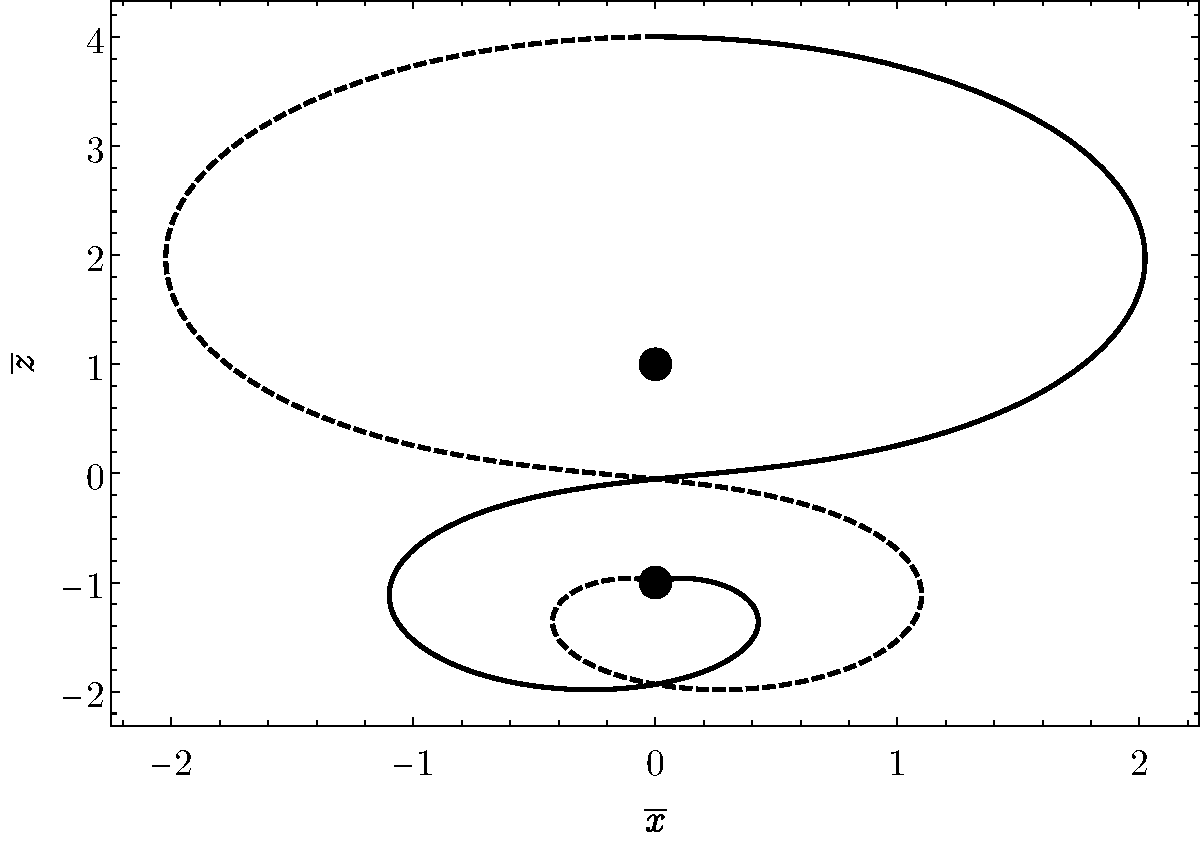
\includegraphics[width = 0.51\linewidth]{img/penrose_binaries/mp/orbit_1.pdf}
        \label{ch:penrose_binaries/fig:orbit_1}
    }
    \subfloat[$\overline{\rho}(0) = 0$, $\overline{z}(0) = 4.06$, $\dot{\overline{z}} = 0$, $E = -1$, $\mu = -9.63222$]{
        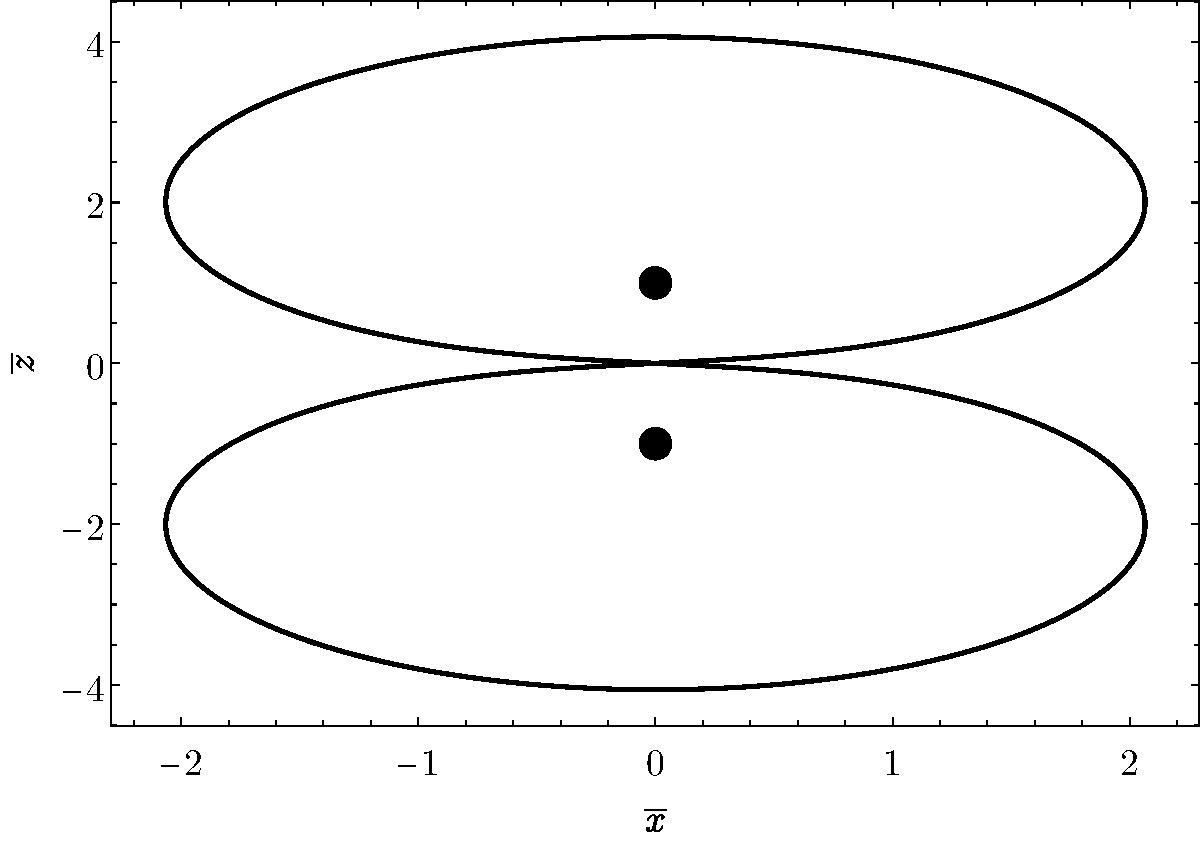
\includegraphics[width = 0.51\linewidth]{img/penrose_binaries/mp/orbit_2.pdf}
        \label{ch:penrose_binaries/fig:orbit_2}
    }
    \caption{Two different types of orbits in the $\rho$-$z$ plane: terminating (left) and closed (right). Initial conditions used for each orbits are presented in their respective captions. The dashed trajectory represents that of negative $\dot{\overline{\rho}}(0)$.}
    \label{ch:penrose_binaries/fig:rho_z_orbits}
\end{figure}

\subsubsection{Orbits in the $z=0$ plane}

If we set $z(0) = \dot{z}(0) = 0$ we confine the particle's motion to the plane exactly in between the two black holes and once the background spacetime parameters have been set the trajectory can now be readily determined using only Eq.~\eqref{ch:penrose_binaries/eq:first_order_ode_for_orbits} with appropriate values for $\rho(0)$, $\phi(0)$, $L$, $E$ and $\mu$. Thanks to the constrained motion we can now take full advantage of the effective potential formulation that we've introduced earlier. Our search revealed that particles with negative energy in this plane stay in a perpetual oscillatory motion either in straight lines or more complicated precessing orbits, depending on the value of $L$. These oscilating orbits are similar in nature to the closed orbits found in the $\rho$-$z$ plane as they also don't fall towards either of the black holes but they are stable in the sense that they do not require any fine tuning of the orbital parameters to be found, although they are globally unstable as any perturbation along the $z$ direction will cause the to fall towards one of the black holes. Proceeding with the same rescaling by $M_1$ scheme we've adopted so far, we plot in Figs.~\ref{ch:penrose_binaries/fig:orbit_z_1} and \ref{ch:penrose_binaries/fig:orbit_z_2} two oscillating orbits for a binary system with $M = \alpha = 1$. Note that if an infinite amount of time s allowed to pass, a particle following these trajectories will have swept the whole finite area between the minimum and maximum values attained by $\overline{\rho}$ during motion.

It's very hard (or even impossible) to obtain the orbital turning points of any oscilating orbit analytically by solving $E_{\text{eff}}(\rho,0)^2 - V_{\text{eff}}(\rho,0) = 0$ for $\rho$ as one can show that the problem reduces to finding the roots of a sixth-order polynomial equation. Despite that, its quite easy to find the roots of the polynomial numerically after the orbital parameters have been chosen and thus this is the approach we've adopted as a complete and rigorous analysis of the orbital turning points go beyond the scope of this work. In Figs.~\ref{ch:penrose_binaries/fig:veff_for_3} and \ref{ch:penrose_binaries/fig:veff_for_4} we plot the squared effective energy and the effective potential to the orbits described by \ref{ch:penrose_binaries/fig:orbit_z_1} and \ref{ch:penrose_binaries/fig:orbit_z_2} respectively and give their turning points. The effective potential is represented by a solid black line while the squared effective energy is represented by a dashed red line.

\begin{figure}[!htbp]
    \centering
    \subfloat[$\overline{\rho}(0) = 2$, $\phi(0) = 0$, $L = 2$, $E = -1$ and $\mu = -4$.]{
        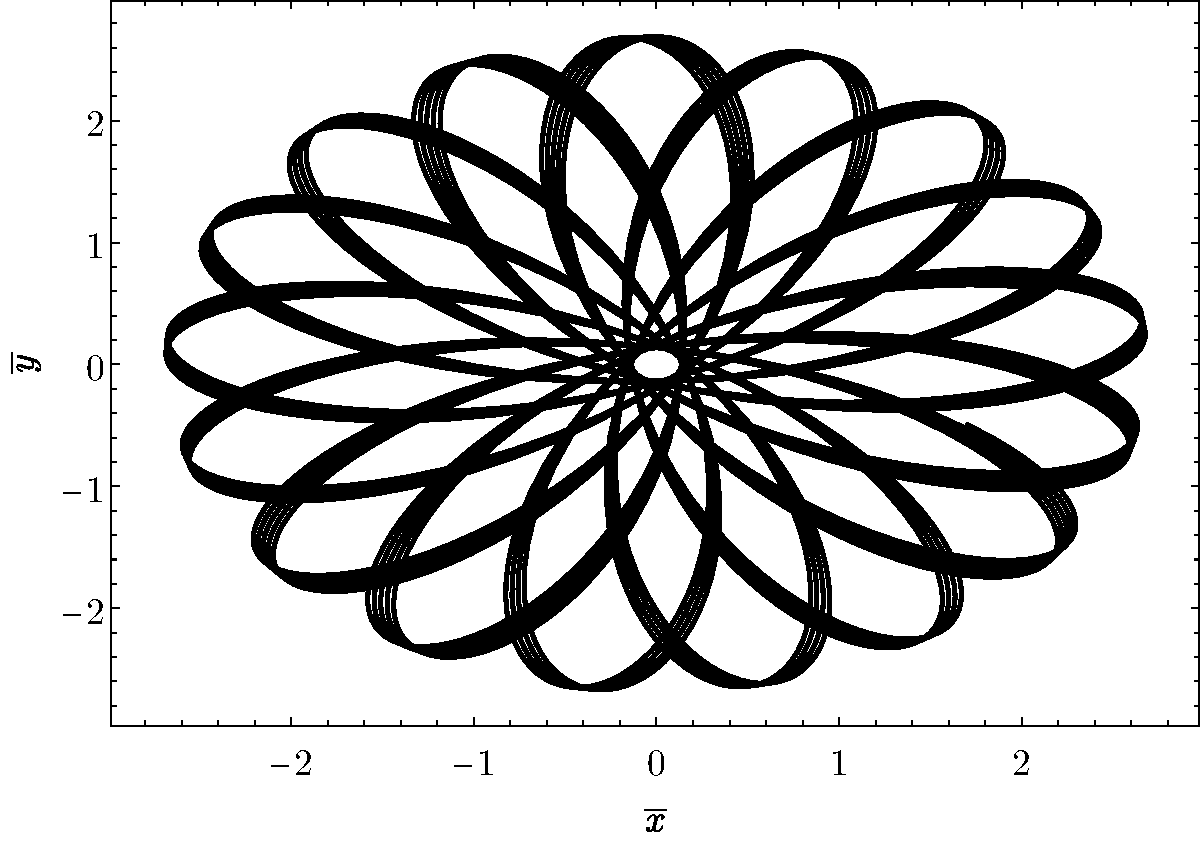
\includegraphics[width = 0.5\linewidth]{img/penrose_binaries/mp/orbit_3.pdf}
        \label{ch:penrose_binaries/fig:orbit_z_1}
    }
    \subfloat[$\overline{\rho}(0) = 2$, $\phi(0) = 0$, $L = 10$, $E = -1$ and $\mu = -6$.]{
        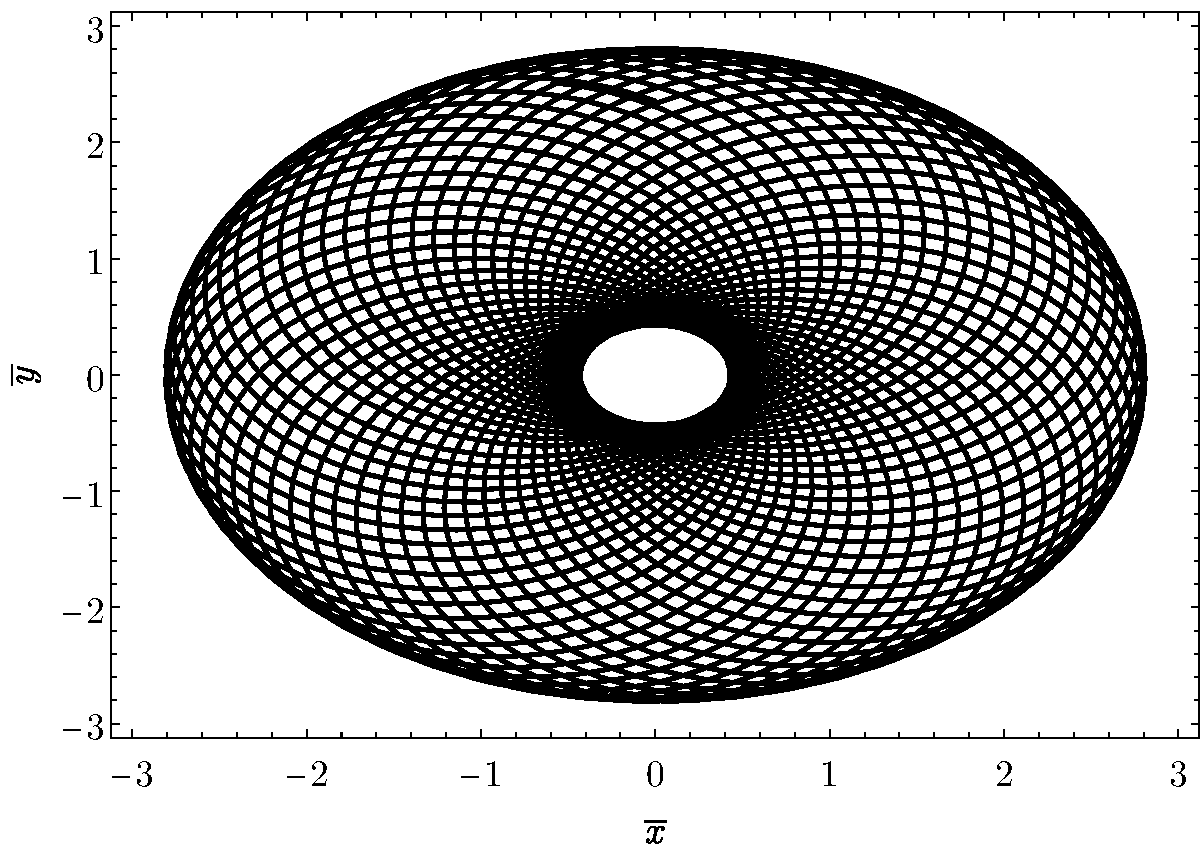
\includegraphics[width = 0.5\linewidth]{img/penrose_binaries/mp/orbit_4.pdf}
        \label{ch:penrose_binaries/fig:orbit_z_2}
    }
    \caption{Two oscilating orbits in the $z = 0$ symmetry plane. Note that the area swept by a particle in either orbit after an infinite amount of time is finite and proportional to the difference between the and outer orbital radii.}
    \label{ch:penrose_binaries/fig:z_orbits}
\end{figure}

\begin{figure}[!htbp]
    \centering
    \subfloat[Turning points: $\overline{\rho}_{\text{min}} = 0.1386$ and $\overline{\rho}_{\text{max}} = 2.6883$.]{
    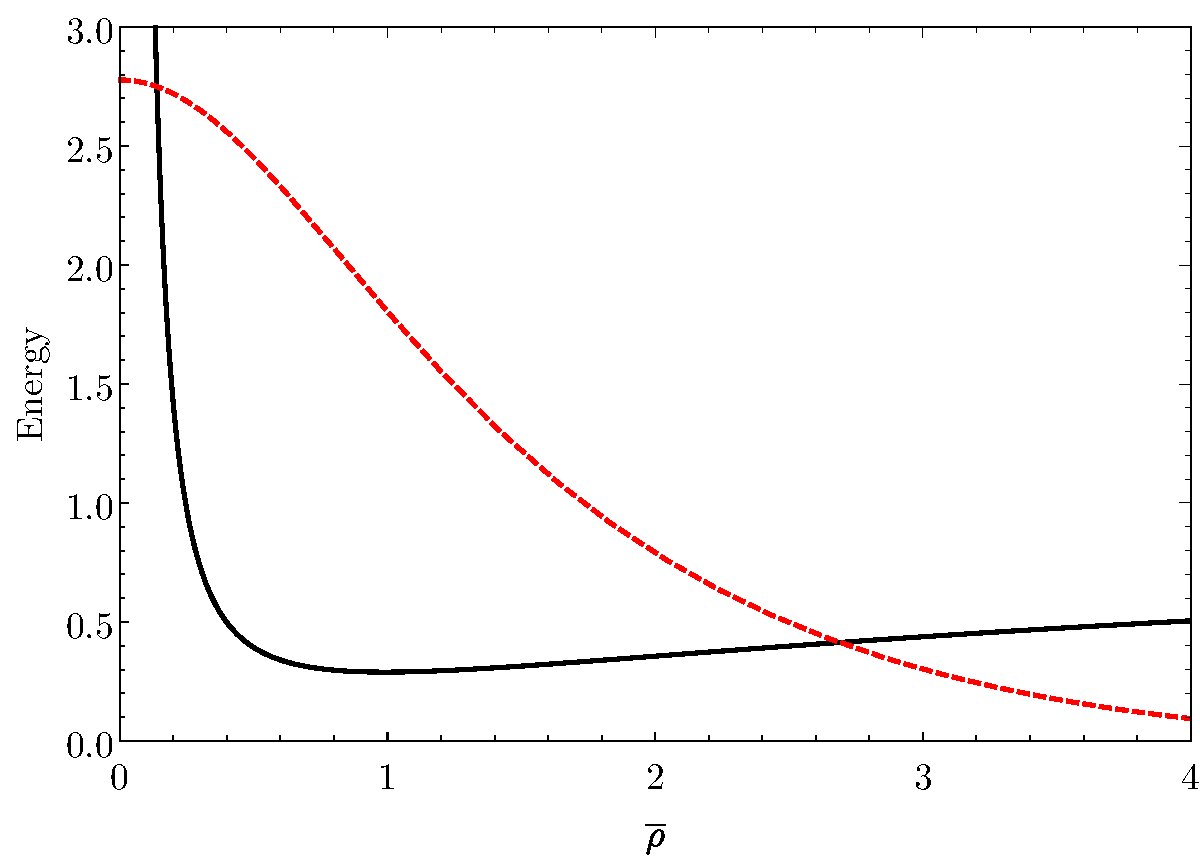
\includegraphics[width = 0.5\linewidth]{img/penrose_binaries/mp/veff_for_3.pdf}
    \label{ch:penrose_binaries/fig:veff_for_3}
    }
    \subfloat[Turning points: $\overline{\rho}_{\text{min}} = 0.4352$ and $\overline{\rho}_{\text{max}} = 2.8091$.]{
    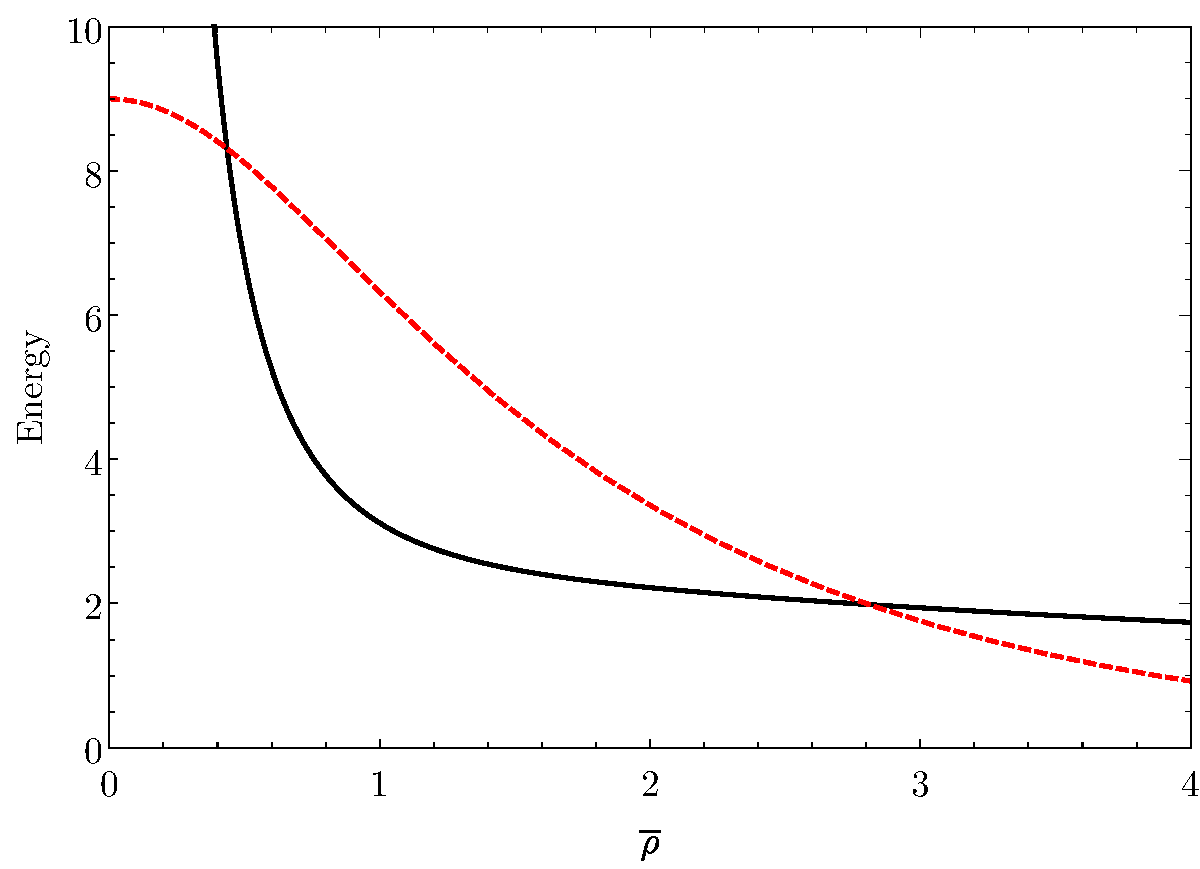
\includegraphics[width = 0.5\linewidth]{img/penrose_binaries/mp/veff_for_4.pdf}
    \label{ch:penrose_binaries/fig:veff_for_4}
    }
    \caption{The effective potential (solid black line) and squared effective energy (dashed red line) for the orbits depicted in \ref{ch:penrose_binaries/fig:orbit_z_1} (left) and \ref{ch:penrose_binaries/fig:orbit_z_2} (right).}
    \label{ch:penrose_binaries/fig:veff_graphs}
\end{figure}

\subsection{Examples of Penrose processes}

Let us now give concrete examples of energy extraction in a binary black hole spacetime. As we've already seen, under a few different circumstances such as when the black holes are sufficiently apart, the charge-to-mass ratios of the fragments are sufficiently small or when the mass ratio is large, the ergosphere is composed by two disconnected regions. When this happens, the only way to extract energy from the binary is by having the negative energy trajectory reaching the event horizon of one of the black holes. Consequently, the negative energy particle will eventually reach one of the singularities. If, on the other hand, the black holes are sufficiently close to each other, an interesting possibility opens up. Instead of having the negative energy orbit reach one of the event horizons, we can engineer the break up so that it will exist forever outside the black holes, confined to the ergosphere of the binary using trajectories like those in Figs.~\ref{ch:penrose_binaries/fig:orbit_2}, \ref{ch:penrose_binaries/fig:orbit_z_1} or \ref{ch:penrose_binaries/fig:orbit_z_2}. Naturally, $T^{(1)}$ (the negative energy trajectory) will only make sense physically if $\dot{\rho}^2 \ge 0$ everywhere. Thus, once $E^{(1)}$ and $L^{(1)}$ have been specified, the requirement that\label{ch:penrose_binaries/eq:effective_potential_orbit_equation} be non-negative constrains the possible value for the break-up coordinate $\rho_0$. Note that the angular break-up coordinate $\phi_0$ is irrelevant due to the system being symmetric with respect to rotations around the $z$ axis.

To construct an example, we start of by selecting a negative energy trajectory $T^{(1)}$ and a break-up point inside the ergosphere. After that, we construct an arbitrary orbit of positive energy that reaches infinity to serve as $T^{(2)}$. By solving the system formed by Eqs.~\eqref{ch:penrose_binaries/eq:four_momentum_conservation}-\eqref{ch:penrose_binaries/eq:conservation_rho} together with the conservation of electric charge, one is able to determine all of the orbital parameters for $T^{(0)}$. In Table~\ref{ch:penrose_binaries/tab:exemple_orbital_parameters_1} we summarize the orbital parameters for the process depicted in Fig. \ref{ch:penrose_binaries/fig:penrose_example_1}. The particle comes in orbit $T^{(1)}$ represented by the solid black curve and then splits at the grey dot into a negative energy orbit $T^{(1)}$ represented by a blue dotted curve and a positive energy orbit $T^{(2)}$ represented by a red dashed curve. In this example, we've set the spacetime parameters at $M = \alpha = 1$ and the two black dots represent the black hole's event horizons. Note that the entire process is confined to the $\rho$-$z$ plane.

\begin{table}[!htbp]
    \centering
    \caption{Orbital parameters for an example Penrose process in the $\rho$-$z$ plane.}
    \begin{tabular}{c|c|c|c|c|c|c|c|}
        \cline{1-8}
        \multicolumn{1}{|c|}{$T^{(i)}$} & $\mu^{(i)}$ & $E^{(i)}$ & $L^{(i)}$ & $\rho_0^{(i)}$ & $z_0^{(i)}$ & $\dot{\rho}_0^{(i)}$ & $\dot{z}_0^{(i)}$ \\ \hline
        \multicolumn{1}{|c|}{$T^{(0)}$} & $0.16076$   & $3.93401$ & $0$       & $0$            & $4.06$      & $3.82283$            & $0$               \\ \hline
        \multicolumn{1}{|c|}{$T^{(1)}$} & $-9.63222$  & $-1$      & $0$       & $0$            & $4.06$      & $-2.21869$           & $0$               \\ \hline
        \multicolumn{1}{|c|}{$T^{(2)}$} & $10$        & $10$      & $0$       & $0$            & $4.06$      & $6.52697$            & $0$               \\ \hline
    \end{tabular}
    \label{ch:penrose_binaries/tab:exemple_orbital_parameters_1}
\end{table}

\begin{figure}[!htbp]
    \centering
    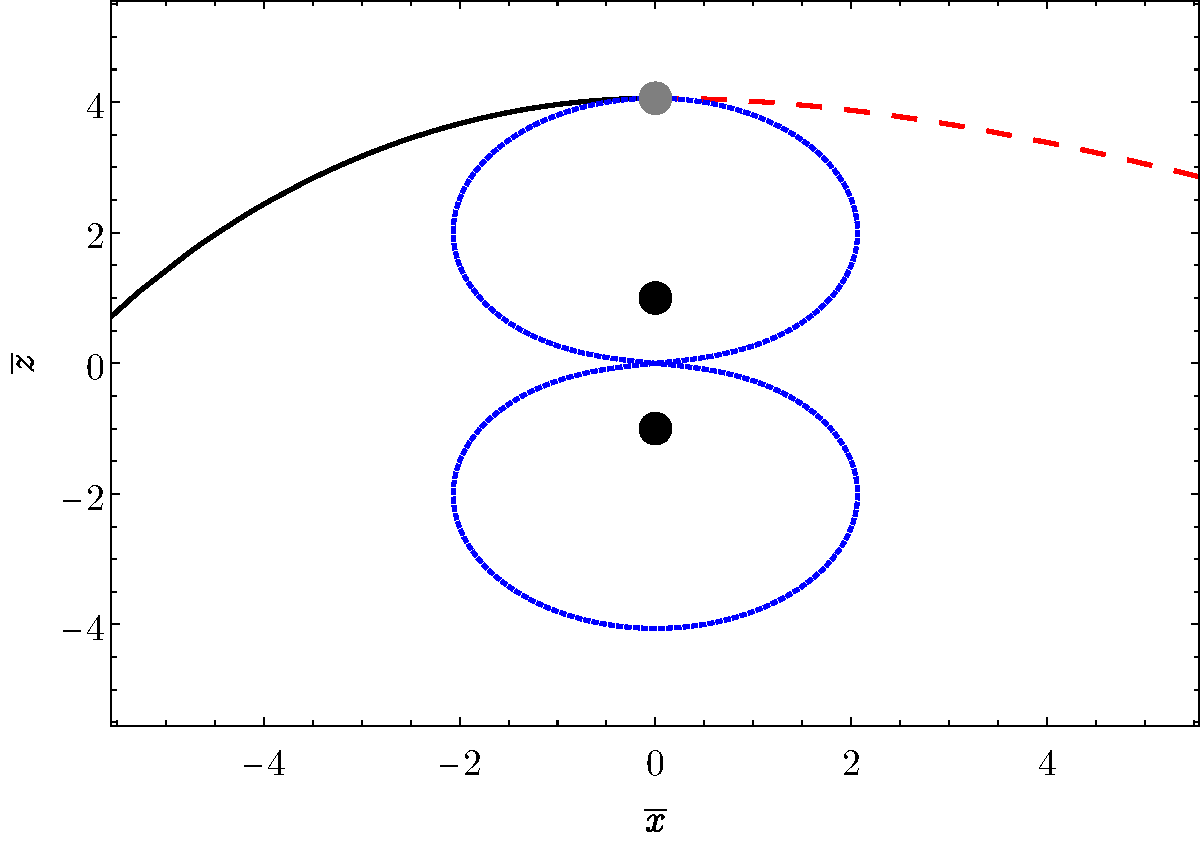
\includegraphics[scale = 0.4]{img/penrose_binaries/mp/penrose_xz.pdf}
    \caption{Example of a penrose process in the $\rho$-$z$ plane. The incoming trajectory (solid black) splits at the grey point into an negative energy (dotted blue) and increased energy (dashed red) orbit.}
    \label{ch:penrose_binaries/fig:penrose_example_1}
\end{figure}

If instead we choose to confine our orbits to the $z=0$ plane, by employing the same algorithm with the same background spacetime parameters as before, we obtain the orbital parameters described in Tab.~\ref{ch:penrose_binaries/tab:exemple_orbital_parameters_2} and depicted in Fig. \ref{ch:penrose_binaries/fig:penrose_example_2}. Here we've chosen to draw only a few periods of the oscilating trajectory $T^{(1)}$ to improve the figure's clarity.

\begin{table}[!htbp]
    \centering
    \caption{Orbital parameters for an example Penrose proces in the $z=0$ plane.}
    \begin{tabular}{c|c|c|c|c|c|c|c|}
        \cline{1-8}
        \multicolumn{1}{|c|}{$T^{(i)}$} & $\mu^{(i)}$ & $E^{(i)}$ & $L^{(i)}$ & $\rho_0^{(i)}$ & $z_0^{(i)}$ & $\dot{\rho}_0^{(i)}$ & $\dot{z}_0^{(i)}$ \\ \hline
        \multicolumn{1}{|c|}{$T^{(0)}$} & $-0.85050$  & $2.18701$ & $1.70101$ & $2$            & $0$         & $2.52301$            & $0$               \\ \hline
        \multicolumn{1}{|c|}{$T^{(1)}$} & $-4$        & $-1$      & $2$       & $2$            & $0$         & $-0.65820$           & $0$               \\ \hline
        \multicolumn{1}{|c|}{$T^{(2)}$} & $0.5$       & $10$      & $4$       & $2$            & $0$         & $-9.72474$           & $0$               \\ \hline
    \end{tabular}
    \label{ch:penrose_binaries/tab:exemple_orbital_parameters_2}
\end{table}

\begin{figure}[!htbp]
    \centering
    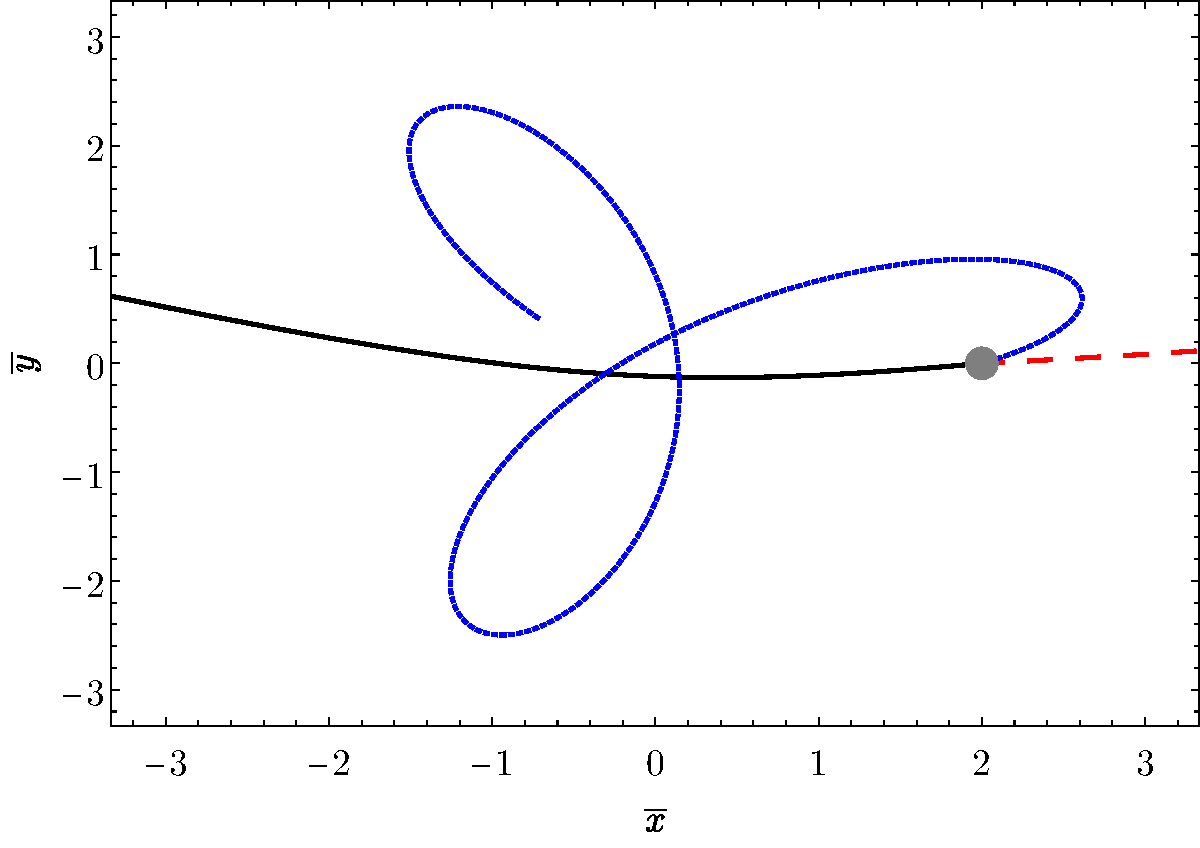
\includegraphics[scale = 0.43]{img/penrose_binaries/mp/penrose_xy.pdf}
    \caption{Example of a Penrose process that happens entirely on the $z=0$ plane of a MP binary black hole. Once again, the incoming trajectory (solid black) splits at the grey point into an negative energy (dotted blue) and increased energy (dashed red) orbit.}
    \label{ch:penrose_binaries/fig:penrose_example_2}
\end{figure}

\subsection{Efficiency of energy extraction}

The efficiency $\eta$ of the Penrose process can be trivially defined as the ratio between the energy input and output. Using Eq.~\eqref{ch:penrose_binaries/eq:conservation_of_charge_energy}, we can see that

\begin{equation}
    \eta = - \frac{m^{(1)}}{m^{(0)}} \frac{E^{(1)}}{E^{(0)}}.
    \label{ch:penrose_binaries/eq:penrose_efficiency_general}
\end{equation}

One can choose $E^{(1)} = 1$ and $m^{(1)}/m^{(0)} = 1$ without any loss of generality. Furthermore it's clear that in order to obtain maximum efficiency, one must choose $E^{(1)}$ to be as negative as possible, and thus of the form of Eq.~\eqref{ch:penrose_binaries/eq:minimum_energy}. With these choices, the efficiency becomes

\begin{equation}
    \eta = \mu^{(1)}\left(\frac{1}{U} - 1\right) - \frac{1}{U}.
    \label{ch:penrose_binaries/eq:penrose_efficiency_max}
\end{equation}

Notice that because \eqref{ch:penrose_binaries/eq:penrose_efficiency_max} depends on $U$, the efficiency depends on the particle's position. Using spherical coordinates centered around the origin, one can see that as $a\rightarrow 0$,

\begin{equation}
    \eta = -\frac{\mu^{(1)}(M_1 + M_2) + r}{M_1 + M_2 + r},
    \label{ch:penrose_binaries/eq:a_zero_efficiency}
\end{equation}
%
which is precisely the efficiency one would obtain for and extremal RN black hole of mass $M_1 + M_2$ in a coordinate system where the event horizon is a point. If the particle is locate precisely at the event horizon, and thus $r = 0$, the efficiency attains it's maximum value of $-\mu^{(1)}$. The direct consequence of this fact is that one can have Penrose processes in which the efficiency of energy extraction goes above 100\% (as $\mu^{(1)}$ can be arbitrarily large) if the participating particles are electrically charged, a well know fact pointed out in Refs.~\cite{bhat1985energetics} and \cite{parthasarathy1986high}.

Additionally, because $0 \leq 1/U \leq 1$, one can easily see from Eq.~\eqref{ch:penrose_binaries/eq:penrose_efficiency_max} that $0 \leq \eta \leq -\mu^{(1)}$ and thus the presence of the second black hole does not allow for more efficient processes than the single RN black hole. It's also noteworthy that $\eta$ attains it's maximum value when $1/U = 0$ which occurs only when the particle is exactly over one of the event horizons. In Fig.~\ref{ch:penrose_binaries/fig:efficiency}, we plot the extraction efficiency for a MP binary with mass ratio $M = 1$ and varying separation parameter $\alpha$ for a particle of charge-to-mass ratio $\mu = -1$ located at $\overline{r} = 1$ and $\overline{\theta} = 0$ (solid black line), $\overline{\theta} = \pi/8$ (dashed red line) and $\overline{\theta} = \pi/2$ (dotted blue line). The maximum value of $\alpha$ is caped by the generalized ergosphere condition of Eq.\eqref{ch:penrose_binaries/eq:rescaled_negative_energy_condition}. Note that the maximum efficiency of $-\mu = 2$ is attainable only when the particle is located at one of the event horizons, namely when $\alpha = 1$ and $\overline{\theta} = 0,\pi/2$.

\begin{figure}[!htbp]
    \centering
    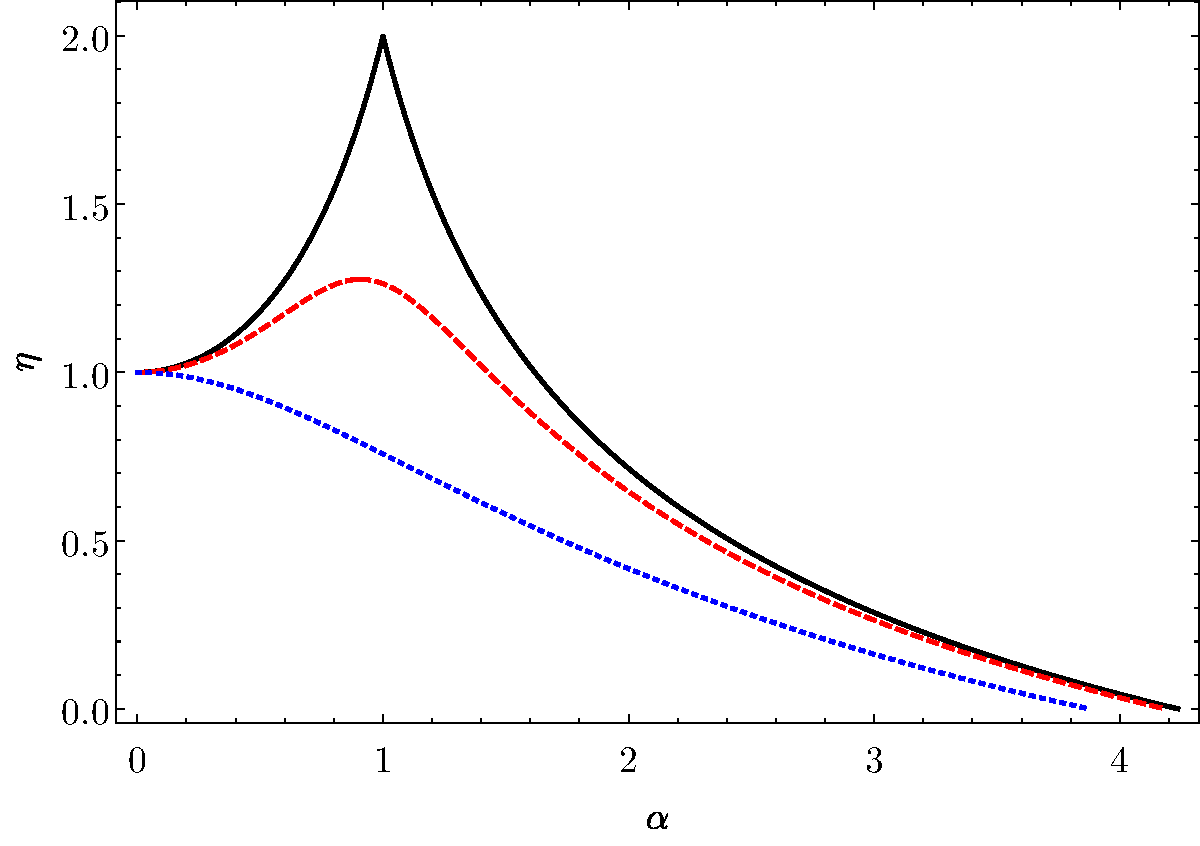
\includegraphics[scale = 0.4]{img/penrose_binaries/mp/efficiency.pdf}
    \caption{Extraction efficiency for a particle $\overline{r} = 1$ and $\overline{\theta} = 0$ (solid black line), $\overline{\theta} = \pi/8$ (dashed red line) and $\overline{\theta} = \pi/2$ (dotted blue line). Maxmimum efficiency is attained at $\alpha = 1$ and $\overline{\theta} = 0,\pi/2$.}
    \label{ch:penrose_binaries/fig:efficiency}
\end{figure}